% fig03_penning_spectrum.tex — Penning-trap eigenfrequency spectrum (log scale).
% Compiled by the paper Makefile via `make figures` (pdflatex on the snippet).
%
% Data: §Penning keystone + companion/verify-ledger.json (penning_* atoms).
% Representative antiproton trap B=5T, U0=10V, d=5mm, m=m_p (CPT).
%   f_+ (modified cyclotron) ~ 76.22 MHz = 7.622e7 Hz
%   f_z (axial)             ~ 985 kHz    = 9.85e5 Hz
%   f_- (magnetron)         ~ 6.37 kHz   = 6.37e3 Hz
% The three span ~4 decades; the invariance theorem ties them to f_c.
%
% Manual single-shot compile (debug):
%   pdflatex -interaction=nonstopmode -halt-on-error fig03_penning_spectrum.tex
\documentclass[border=4pt]{standalone}
\usepackage{tikz}
\usepackage{pgfplots}
\pgfplotsset{compat=1.18}
\begin{document}
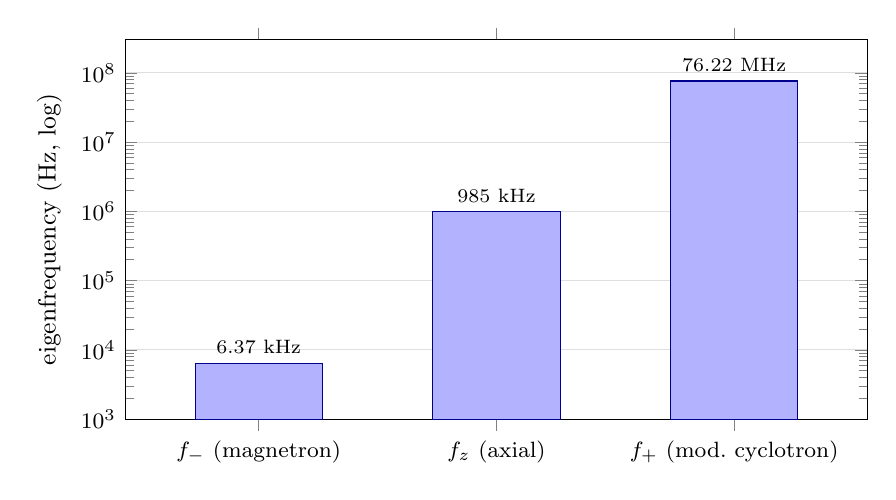
\begin{tikzpicture}
\begin{axis}[
  width=11cm, height=6.4cm,
  ybar,
  bar width=46pt,
  ymode=log,
  log origin=infty,
  ymin=1e3, ymax=3e8,
  ylabel={eigenfrequency (Hz, log)},
  symbolic x coords={magnetron, axial, cyclotron},
  xtick={magnetron, axial, cyclotron},
  xticklabels={$f_-$ (magnetron), $f_z$ (axial), $f_+$ (mod.\ cyclotron)},
  tick label style={font=\footnotesize},
  label style={font=\small},
  nodes near coords,
  nodes near coords style={font=\scriptsize},
  point meta=explicit symbolic,
  ymajorgrids,
  grid style={gray!25},
  enlarge x limits=0.28,
]
\addplot[draw=blue!55!black,fill=blue!30] coordinates {
  (magnetron, 6.37e3) [6.37 kHz]
  (axial,     9.85e5) [985 kHz]
  (cyclotron, 7.622e7)[76.22 MHz]
};
\end{axis}
\end{tikzpicture}
\end{document}
